\documentclass[aspectratio=169]{beamer}

\usepackage{amsmath, amssymb, bm}
\usepackage{cancel}
\usepackage{tikz}
\usetikzlibrary{arrows.meta,calc,positioning,bending}

\definecolor{mygreen}{RGB}{0,110,20}
\definecolor{myorange}{RGB}{240,120,0}
\definecolor{mygray}{RGB}{120,120,120}
\definecolor{boxgray}{RGB}{150,150,150}
\definecolor{axisgray}{RGB}{40,60,65}
\definecolor{citegray}{RGB}{165,165,165}

\makeatletter
\renewcommand{\@cite}[2]{{\color{citegray}\footnotesize(#1\if@tempswa, #2\fi)}}
\makeatother


\usetheme[
  style=minimal,
  palette=horizon,
  frametitle=subtle,
  progressbar,
  sansface={libertinus},
%   mathface=libertinus,
]{Celestia}



\AtBeginDocument{\hypersetup{colorlinks=true,allcolors=citegray,citecolor=citegray}}

\title{Macroeconomics in the Sequence Space}
\author{Chen Gao \and Weigao Wang}
\institute{School of Economics, Peking University}
\date{\today}


\begin{document}

\maketitle

\begin{frame}{Outline}
    \tableofcontents
\end{frame}

\small

\section{Why Sequence Space?}

\begin{frame}{Sequence Space vs.\ State Space}{Motivation}

    \begin{itemize}
        \item In heterogeneous-agent (HA) models, the economy’s state is the \alert{entire cross-sectional distribution} — an infinite-dimensional object.
        \item Sequence-space methods \emph{sidestep} this challenge: they characterize \alert{local dynamics around the steady state} without ever carrying the distribution as a state variable.
        \item The key insight: aggregate equilibrium dynamics can be represented in sequence space as mappings from \alert{aggregate shock paths} to \alert{aggregate outcomes}, with Jacobians arising as the local linear approximation of these mappings.
    \end{itemize}

\end{frame}


\begin{frame}{Sequence Space vs.\ State Space}{State Space}

    \begin{definition}
        A \alert{state-space representation} describes the economy recursively.
        At date $t$, a state variable $x_t$ summarizes all payoff-relevant history, and the model evolves as
        \[
            x_{t+1}=f(x_t,\varepsilon_{t+1}),
            \qquad
            y_t=g(x_t).
        \]
        \emph{Given $x_t$, the future is independent of the past.}
    \end{definition}
\end{frame}

\begin{frame}{Sequence Space vs.\ State Space}{Sequence Space}

    \begin{definition}
        A \alert{sequence-space representation} characterizes equilibrium as a mapping between entire time paths. We seek sequences $\{X_t\}_{t=0}^{\infty}$ such that equilibrium conditions hold at every date:
        \[
            F\!\left(\{X_t\}_{t=0}^{\infty},\{Z_t\}_{t=0}^{\infty}\right)=\bm{0},
        \]
        where $\{X_t\}$ collects endogenous variables and $\{Z_t\}$ collects exogenous shocks or policy paths.
    \end{definition}

\end{frame}


\begin{frame}{Sequence Space vs.\ State Space}{Comparison}

    \begin{block}{Intuition}
        \begin{itemize}
            \item State space asks: \emph{what is the current state, and how does it transition?}
            \item Sequence space asks: \emph{given a shock path, what equilibrium outcome path clears all markets?}
        \end{itemize}
    \end{block}

    \begin{block}{Takeaway}
        When the distribution is the intractable state variable, sequence space replaces a high-dimensional state-space problem with a representation in terms of \alert{equilibrium mappings over aggregate paths}, making analysis and computation much more tractable.
    \end{block}
\end{frame}



\section{Local Solution}


\subsection{SSJ}
\begin{frame}{Steady State}{The Standard Incomplete Markets Model}
    Core of the canonical HA model: the SIM model
    \begin{align}
        V_t (s, a) & = \max_{c,\, a'} \; u (c) + \beta \mathbb{E} \left[ V_{t+1} (s', a') \mid s \right], \label{eq:sim-bellman} \\
        \text{s.t.} \quad & a' + c = (1 + r_t) a + y_t (s) \\
        & a' \geq a
    \end{align} 

    We basically need 4 steps to solve the steady state:
    \begin{enumerate}
        \item Discretize the state space
        \item Solve for steady state policy functions $a'(s, a)$ and $c(s, a)$
        \item Solve for steady state distribution $D(s, a)$
        \item Aggregate assets and consumption
    \end{enumerate}
\end{frame}


\begin{frame}{Steady State}{Step 1: Discretization}
    \textbf{Asset Grid for $a$:}
    \begin{itemize}
        \item It is common to use a uniform grid.
        \item Most nonlinearity occurs near the borrowing constraint $a$, so more points should be placed close to the constraint.
        \item \textbf{Solution:} Use a double exponential grid:
        \[
            a_i = \underline{a} + \exp\left(\exp(u_i) - 1\right) - 1
        \]
        where $u_i$ is uniform on $[0, \bar{u}]$.
    \end{itemize}
    \textbf{Markov Chain for $s$:}
    \begin{itemize}
        \item Approximate an AR(1) process with persistence $\rho$.
        \item For $\rho \approx 1$, use Rouwenhorst’s method.
    \end{itemize}
\end{frame}

\begin{frame}{Steady State}{Step 2: Steady State policies}
    We'll use two optimality conditions: 

    \textbf{Envelope Condition:}
    \begin{equation}
        V_{a,t}\left(s,a\right) = \left( 1 + r_{t} \right) u'\left(c_{t}\left(s,a\right)\right)\label{eq:sim-envelope}
    \end{equation}

    \textbf{First Order Condition:}
    \begin{equation}
        u'\left( c_{t}\left( s, a \right) \right) \geq \beta \mathbb{E}\left[ V_{a,t+1}\left( s', a_{t}^{\prime}\left( s, a \right) \right) \right]\label{eq:sim-foc}
    \end{equation}
    with equality unless the budget constraint binds.

\vspace{0.5em}
    The key to solving for steady state policies is to use \textbf{EGM} backward iteration. Each iteration proceeds as follows:
    \[
        V_{a,t+1}\left( s', a' \right)
        \xrightarrow{\eqref{eq:sim-foc}} 
        c_{t}^{\text{endo}}\left( s, a' \right)
        \xrightarrow{\text{interpolate}} 
        a_{t}'\left( s, a \right)
        \xrightarrow{\eqref{eq:sim-bellman}} 
        c_{t}\left( s, a \right)
        \xrightarrow{\eqref{eq:sim-envelope}} 
        V_{a,t}\left( s, a \right)
    \]
\end{frame}


\begin{frame}{Steady State}{Step 3: Distribution}
    \textbf{Goal:} Update the next period distribution $D_{t+1}(s, a)$ using the policy function $a'_t(s, a)$.

    \textbf{Issue:} The policy $a'_t(s, a)$ generally \alert{does not land exactly on the grid points}.


    \vspace{0.5em}


    \textbf{Solution:} Use \alert{lotteries} to distribute probability mass. The idea is to map the current mass to adjacent grid points in the next period based on interpolation weights.


    \vspace{0.5em}

    Suppose for two grid points $a_i$, $a_{i+1}$, the policy yields:
    \[
        a'_t(s, a) = \pi a_i + (1 - \pi) a_{i+1}
    \]
    where $0 \leq \pi \leq 1$. Then, send mass $\pi D_t(s, a)$ to $(s', a_i)$ and $(1 - \pi) D_t(s, a)$ to $(s', a_{i+1})$.


    \vspace{0.5em}

    \textbf{Key Idea:} No simulation is needed! We iteratively update the distribution until it converges.

\end{frame}

\begin{frame}{Steady State}{Step 4: Aggregation}
    For each period $t$, the aggregate variables are easily obtained from the distribution and policy functions:
    \begin{align*}
        C_t &= \sum_{s,a} c_t(s, a) \cdot D_t(s, a) \\
        A_t &= \sum_{s,a} a'_t(s, a) \cdot D_t(s, a)
    \end{align*}
\end{frame}



\begin{frame}{Computing HA Jacobians: the “fake news” algorithm}{Partial Equilibrium Dynamics}

    \textbf{Q:} Given time-varying $\{r_t\}_{t=0}^T$ or $\{y_t(s)\}_{t=0}^T$, how to get $C_t$, $A_t$?


    \vspace{0.5em}

    \textbf{A:} Backward and Forward Iteration!
    \begin{enumerate}
        \item From $V_{a,T} = V_{a,\mathrm{ss}}$, iterate \textbf{backward} to get $a'_t(s,a)$, $c_t(s,a)$ for all $t \geq 0$.
        \item From $D_0(s,a) = D_{\mathrm{ss}}(s,a)$, iterate \textbf{forward} to get $D_t(s,a)$ from $a'_t(s,a)$.
        \item Compute
        \[
            C_t = \sum_{s,a} c_t(s,a) \cdot D_t(s,a), \qquad
            A_t = \sum_{s,a} a'_t(s,a) \cdot D_t(s,a)
        \]
    \end{enumerate}

\end{frame}


\begin{frame}{Computing HA Jacobians: the “fake news” algorithm}{Partial Equilibrium Dynamics}
    \centering
    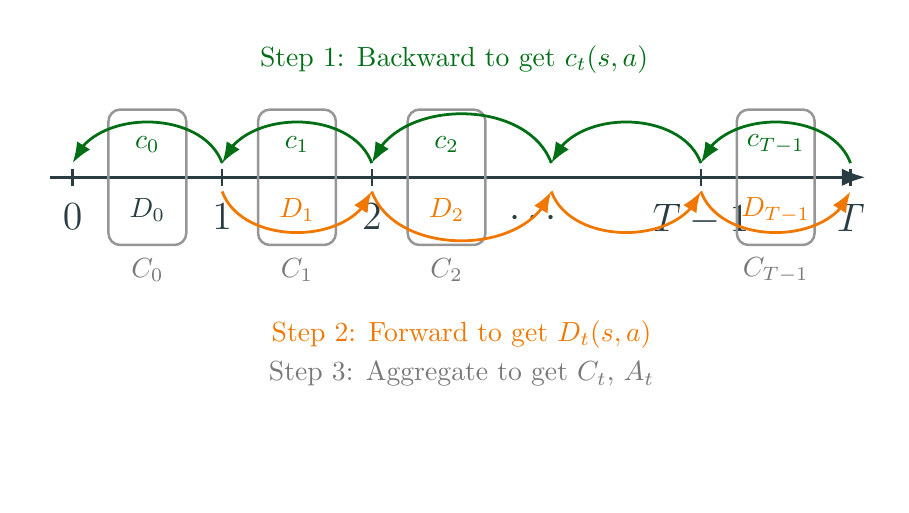
\begin{tikzpicture}[x=1.9cm,y=1cm,>=Latex,thick]
        \path[use as bounding box] (-0.3,-3.9) rectangle (5.4,1.9);

        % ---------- colors ----------


        % ---------- timeline ----------
        \draw[axisgray, line width=1.1pt, -{Latex[length=3mm]}] (-0.15,0) -- (5.30,0);

        % ticks
        \foreach \x in {0,1,2,4.2,5.2}{
                \draw[axisgray, line width=0.9pt] (\x,0.11) -- (\x,-0.11);
            }

        % labels
        \node[below=6pt, text=axisgray] at (0,0) {\Large $0$};
        \node[below=6pt, text=axisgray] at (1,0) {\Large $1$};
        \node[below=6pt, text=axisgray] at (2,0) {\Large $2$};
        \node[below=6pt, text=axisgray] at (4.2,0) {\Large $T-1$};
        \node[below=6pt, text=axisgray] at (5.2,0) {\Large $T$};
        \node[text=axisgray] at (3.1,-0.52) {\Large $\cdots$};

        % ---------- boxes ----------
        \def\boxw{0.52}
        \def\boxh{1.72}

        % t=0
        \draw<4->[rounded corners=0.15cm, boxgray, line width=0.9pt]
        (0.5-\boxw/2,-\boxh/2) rectangle (0.5+\boxw/2,\boxh/2);
        \node<2->[text=mygreen] at (0.5,0.42) { $c_0$};
        \node<3->[text=axisgray] at (0.5,-0.42) { $D_0$};
        \node<4->[text=mygray] at (0.5,-1.18) { $C_0$};

        % t=1
        \draw<4->[rounded corners=0.15cm, boxgray, line width=0.9pt]
        (1.5-\boxw/2,-\boxh/2) rectangle (1.5+\boxw/2,\boxh/2);
        \node<2->[text=mygreen] at (1.5,0.42) { $c_1$};
        \node<3->[text=myorange] at (1.5,-0.42) { $D_1$};
        \node<4->[text=mygray] at (1.5,-1.18) { $C_1$};

        % t=2
        \draw<4->[rounded corners=0.15cm, boxgray, line width=0.9pt]
        (2.5-\boxw/2,-\boxh/2) rectangle (2.5+\boxw/2,\boxh/2);
        \node<2->[text=mygreen] at (2.5,0.42) { $c_2$};
        \node<3->[text=myorange] at (2.5,-0.42) { $D_2$};
        \node<4->[text=mygray] at (2.5,-1.18) { $C_2$};

        % t=T-1
        \draw<4->[rounded corners=0.15cm, boxgray, line width=0.9pt]
        (4.7-\boxw/2,-\boxh/2) rectangle (4.7+\boxw/2,\boxh/2);
        \node<2->[text=mygreen] at (4.7,0.42) { $c_{T-1}$};
        \node<3->[text=myorange] at (4.7,-0.42) { $D_{T-1}$};
        \node<4->[text=mygray] at (4.7,-1.18) { $C_{T-1}$};

        % =========================================================
        % Step 1: backward
        % =========================================================
        \draw<2->[mygreen, line width=1pt, ->]
            (1,0.18) to[out=110,in=70] (0,0.18);
        \draw<2->[mygreen, line width=1pt, ->]
            (2,0.18) to[out=110,in=70] (1,0.18);

        % the missing arrow from ... to 2
        \draw<2->[mygreen, line width=1pt, ->]
            (3.2,0.18) to[out=110,in=70] (2,0.18);

        \draw<2->[mygreen, line width=1pt, ->]
            (4.2,0.18) to[out=110,in=70] (3.2,0.18);
        \draw<2->[mygreen, line width=1pt, ->]
            (5.2,0.18) to[out=110,in=70] (4.2,0.18);

        \node<2->[mygreen, align=center] at (2.55,1.5)
            {Step 1: Backward to get $c_t(s,a)$};

        % =========================================================
        % Step 2: forward
        % =========================================================
        \draw<3->[myorange, line width=1pt, ->]
            (1,-0.18) to[out=-70,in=-110] (2,-0.18);
        \draw<3->[myorange, line width=1pt, ->]
            (2,-0.18) to[out=-70,in=-110] (3.2,-0.18);
        \draw<3->[myorange, line width=1pt, ->]
            (3.2,-0.18) to[out=-70,in=-110] (4.2,-0.18);
        \draw<3->[myorange, line width=1pt, ->]
            (4.2,-0.18) to[out=-70,in=-110] (5.2,-0.18);

        \node<3->[myorange, align=center] at (2.60,-2)
            {Step 2: Forward to get $D_t(s,a)$};

        % =========================================================
        % Step 3: aggregate
        % =========================================================
        \node<4->[text=mygray, align=center] at (2.60,-2.5)
            {Step 3: Aggregate to get $C_t$, $A_t$};

    \end{tikzpicture}
\end{frame}


\begin{frame}{Computing HA Jacobians: the ``fake news'' algorithm}{Sequence-space Jacobians}

    Denote the impulse response of aggregate consumption $C_t$ to a one-time productivity shock $y_s$ at  time $s$ by:
    \[
        \frac{\partial C_t}{\partial y_s}
    \]
    We want the stacked matrix:
    \[
        \mathcal{J}^{C,y} \equiv \begin{pmatrix} \dfrac{\partial C_t}{\partial y_s} \end{pmatrix}_{T \times T}  =  \begin{pmatrix} \mathcal{J}_{ts}^{C,y} \end{pmatrix}_{T \times T}
    \]
    Such a matrix is the \alert{sequence-space Jacobian (SSJ)}.

\end{frame}



\begin{frame}{Computing HA Jacobians: the ``fake news'' algorithm}{How to compute}
    To compute the SSJ, we truncate to some finite time $T$ (e.g., $T = 300$).


    For a generic approach with $T$ columns, one would need $T^2$ backward iterations and $T^2$ forward iterations. 
    
    \emph{Simply loop over all $s$ and $t$!}

    \vspace{0.5em}


    \textbf{Key result:} This paper computes the SSJ with only $T$ backward and $T$ forward iterations.

\end{frame}

\begin{frame}{Computing HA Jacobians: the ``fake news'' algorithm}{From $\mathcal{O}(T^2)$ to $\mathcal{O}(T)$: First Row}
    Denote by $c_t^s(s,a)$ and $a_t^s(s,a)$ the policies at time $t$ in response to a shock at time $s$.

    \vspace{0.6em}

    \textbf{Key idea 1:} Only the time difference $s-t$ until the perturbation matters.

    \[
    c_t^s(s,a) =
    \begin{cases}
        c_{ss}(s,a) & \text{if } s < t \\[0.8em]
        c_{T-1-(s-t)}^{T-1}(s,a) & \text{if } s \geq t
    \end{cases}
    \]

    \emph{We only compute a single backward iteration with $s = T-1$ to obtain all the $c_t^s(s,a)$.}

    \vspace{0.6em}

    For aggregate responses:
    \begin{itemize}
        \item $C_0^s = \sum_{s,a} c_0^s(s,a)\, D_{ss}(s,a)$, so we get the \alert{first row} of the Jacobian: $\mathcal{J}_{0s}^{C,y} = \dfrac{\partial C_0}{\partial y_s}$.
        \item $D_1^s(s,a)$ is then implied by $c_0^s(s,a)$ for all $s$.
    \end{itemize}
\end{frame}

\begin{frame}{Computing HA Jacobians: the ``fake news'' algorithm}{From $\mathcal{O}(T^2)$ to $\mathcal{O}(T)$: First Column}
    \begin{itemize}
        \item Intuitively, we can continue to compute $D_t^s(s,a)$, then aggregate $c_t^s = c_t^{s'} D_t^s$ for all $s,t$ (Still $O(T^2)!$)
        \item Observe that to first order,
        \[
        dC_t^s = dc_t^{s'} D_{ss} + c_{ss}' dD_t^s
        \]
        \item Consider $s=0$. For $t \geq 1$, only the second term remains,
        \[
        dC_t^0 = \underbrace{\cancel{dc_t^{0'} D_{ss}}}_{c_t^s(s,a)=c_{ss}(s,a),s<t} + c_{ss}' dD_t^0 = c_{ss}' (\Lambda_{ss}')^{t-1} dD_1^0
        \]
        \item Here, $\Lambda_{ss}$ is the steady-state transition matrix for $(s,a)$,\alert{ obtained by $c_{ss}(s,a)$ } so
        \begin{equation}
            dC_t^0 = c_{ss}' (\Lambda_{ss}')^{t-1} dD_1^0 \label{eq:dc_t0}
        \end{equation}
        \item Then we get the \alert{first column} of the Jacobian: $\mathcal{J}_{t0}^{C,y} = \frac{\partial c_t}{\partial y_0}$ by \eqref{eq:dc_t0}.
    \end{itemize}
\end{frame}


\begin{frame}{Computing HA Jacobians: the ``fake news'' algorithm}{From $\mathcal{O}(T^2)$ to $\mathcal{O}(T)$: Fake news for the rest!}
    How about $s > 0$? Given policy symmetry, we have $d\mathbf{c}_t^s = d\mathbf{c}_{t-1}^{s-1}$. It follows:
    \[
        dC_t^s - dC_{t-1}^{s-1} =\cancel{ \left( d\mathbf{c}_t^s - d\mathbf{c}_{t-1}^{s-1} \right)^\prime \mathbf{D}_{ss}}
        +\ \mathbf{c}_{ss}^\prime \left( d\mathbf{D}_t^s - d\mathbf{D}_{t-1}^{s-1} \right)
    \]
    Given \alert{$c_t^s = c_{t-1}^{s-1} \implies \Lambda_t^s = \Lambda_{t-1}^{s-1}$, } it is then easy to see
    \[
        D_t^s - D_{t-1}^{s-1}
        = \prod_{j=1}^{t-1} \left( \Lambda_j^{s\,\prime} \right) \left( \Lambda_0^{s} - I \right)^\prime D_{ss}
        = \prod_{j=1}^{t-1} \left( \Lambda_j^{s\,\prime} \right) ( D_1^s - D_{ss} )
    \]
    Holding $\Lambda_j^{s} \equiv \Lambda_{ss}$, we have
    \begin{equation}
        \mathcal{F}_{ts}\,dy_s \overset{\text{def}}{=}
        \mathbf{c}_{ss}^\prime \left(d\mathbf{D}_t^s - d\mathbf{D}_{t-1}^{s-1}\right)
        = \mathbf{c}_{ss}^\prime \left( \Lambda_{ss}^\prime \right)^{t-1} d\mathbf{D}_1^s
        \equiv \left( \mathcal{J}_{ts}^{C,y} - \mathcal{J}_{t-1,s-1}^{C,y} \right) dy_s \label{eq:fake_news}
    \end{equation}

    We interpret the $\mathcal{F}_{ts}$ as the \textbf{"fake news"} shock on $C_t$:
    \begin{itemize}
        \item[$\bullet$] $t = 0$: news shock that period $s$ shock hits $\Rightarrow d\mathbf{D}_1^s$
        \item[$\bullet$] $t = 1$: fake news that there won't be a shock at $s \Rightarrow c_{ss} \Rightarrow \Lambda_{ss}$ afterwards
    \end{itemize}
\end{frame}


\begin{frame}{Computing HA Jacobians: the ``fake news'' algorithm}{From $\mathcal{O}(T^2)$ to $\mathcal{O}(T)$: Whole $\mathcal{J}^{C,y}$}
    \textbf{Key Idea 2:} Recover $\mathcal{J}^{C,y}$ from 1st row, 1st column and $\mathcal{F}$.

    News shock is a sequence of fake news shocks!

    \[
    \mathcal{J}^{C,y} =
    \begin{pmatrix}
        \mathcal{J}_{00} & \mathcal{J}_{01} & \mathcal{J}_{02} & \dots \\
        \mathcal{J}_{10} & \mathcal{J}_{00} + \mathcal{F}_{00} & \mathcal{J}_{01} + \mathcal{F}_{01} & \dots \\
        \mathcal{J}_{20} & \mathcal{J}_{10} + \mathcal{F}_{10} & \mathcal{J}_{11} + \mathcal{F}_{11} & \dots \\
        \vdots & \vdots & \vdots & \ddots \\
    \end{pmatrix}
    \]

    where, by the recursive structure, representative entries are given by:

    \[
    \mathcal{J}_{ts} =
    \begin{cases}
        \mathcal{J}_{t0} & \text{if } s = 0 \\
        \mathcal{J}_{0s} & \text{if } t = 0 \\
        \mathcal{J}_{t-1,s-1} + \mathcal{F}_{t-1,s-1} & \text{if } t,s \geq 1
    \end{cases}
    \]

\end{frame}


\begin{frame}{Computing HA Jacobians: the ``fake news'' algorithm}{Implementation}
    Define the expectation function:
    \[
        \mathcal{E}_t(s, a) \equiv \mathbb{E} \left[ c_{ss}(s_t, a_t) \mid s_0 = s,\, a_0 = a \right]
    \]
    that is, the expected consumption at time $t$ for an agent starting at $(s,a)$ today.

    \vspace{0.5em}

    This is very easy to compute recursively:
    \[
        \mathcal{E}_0 = c_{ss}, \qquad
        \mathcal{E}_t = \Lambda_{ss} \mathcal{E}_{t-1}
    \]

    \vspace{0.5em}

    \textbf{Key Idea 3:} The $\mathcal{E}_t'$ are enough to get all $t \geq 1$ rows of $\mathcal{F}$:

    \begin{itemize}
        \item \textbf{First column} ($s = 0$): from \eqref{eq:dc_t0},\; $\mathcal{J}_{t0}\, dy_s = \mathcal{E}_t' \, dD^0_1$
        \item \textbf{Other columns} ($s > 0$): from \eqref{eq:fake_news},\; $\mathcal{F}_{ts}\, dy_s = \mathcal{E}_t' \, dD^s_1$
        \item \textbf{Result:} Eventually only $O(T)$ computation!
    \end{itemize}
\end{frame}

\subsection{Theoretical progress after SSJ}

\begin{frame}{DAG}{Krusell-Smith model as a directed acyclic graph (DAG)}
    Recall that we wrote equilibrium in KS model as system

    \[H_t(\bm{K},\bm{Z})\equiv\mathcal{K}_t\left(\left\{ \underbrace{\alpha Z_s K_{s-1}^{\alpha-1}-\delta}_{r_s}, \underbrace{(1-\alpha)Z_s K_{s-1}^\alpha}_{w_s} \right\}_{s=0}^{\infty}\right)-K_t=0\]
where $\mathcal{K}_t \equiv A_t$ is the aggregate capital stock at time $t$ and $\bm{Z} \equiv \{Z_s\}_{s=0}^{\infty}$ is the time-varying TFP process.
    This corresponds to a simple graph:

    \begin{center}
    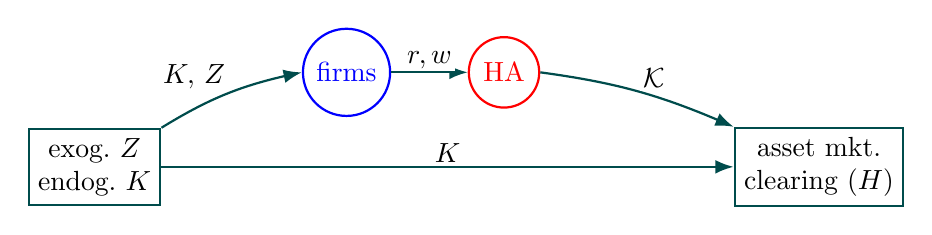
\begin{tikzpicture}[
            >=Latex,
            box/.style={draw=teal!60!black, thick, rectangle,  align=center},
            bluecirc/.style={draw=blue, thick, circle, align=center, text=blue},
            redcirc/.style={draw=red, thick, circle, align=center, text=red},
            flow/.style={->, thick, draw=teal!60!black},
            lab/.style={midway, fill=white, inner sep=1pt}
        ]

        % nodes
        \node[box] (leftbox) at (0,0) {exog.\ $Z$ \\ endog.\ $K$};
        \node[bluecirc] (firms) at (3.2,1.2) {firms};
        \node[redcirc] (ha) at (5.2,1.2) {HA};
        \node[box] (market) at (9.2,0) {asset mkt. \\ clearing $(H)$};

        % arrows
        \draw[flow] (leftbox.north east) to[bend left=10] node[lab, above left] {$K,\,Z$} (firms.west);
        \draw[flow] (firms.east) -- node[lab, above] {$r,w$} (ha.west);
        \draw[flow] (ha.east) to[bend left=8] node[lab,above right] {$\mathcal{K}$} (market.north west);
        \draw[flow] (leftbox.east) -- node[lab, above] {$K$} (market.west);

    \end{tikzpicture}
    \end{center}

\end{frame}

\begin{frame}{DAG}{DAGs combining simple and HA blocks}
    \begin{center}
    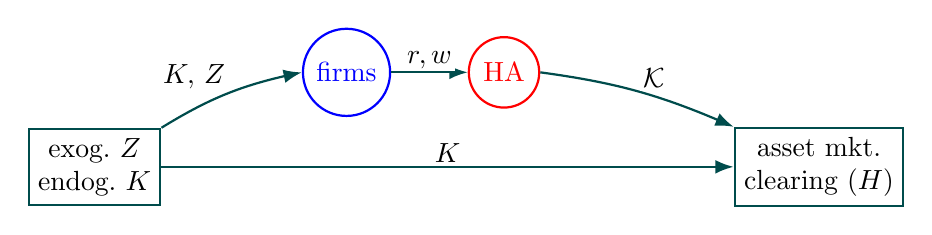
\begin{tikzpicture}[
            >=Latex,
            box/.style={draw=teal!60!black, thick, rectangle,  align=center},
            bluecirc/.style={draw=blue, thick, circle, align=center, text=blue},
            redcirc/.style={draw=red, thick, circle, align=center, text=red},
            flow/.style={->, thick, draw=teal!60!black},
            lab/.style={midway, fill=white, inner sep=1pt}
        ]

        % nodes
        \node[box] (leftbox) at (0,0) {exog.\ $Z$ \\ endog.\ $K$};
        \node[bluecirc] (firms) at (3.2,1.2) {firms};
        \node[redcirc] (ha) at (5.2,1.2) {HA};
        \node[box] (market) at (9.2,0) {asset mkt. \\ clearing $(H)$};

        % arrows
        \draw[flow] (leftbox.north east) to[bend left=10] node[lab, above left] {$K,\,Z$} (firms.west);
        \draw[flow] (firms.east) -- node[lab, above] {$r,w$} (ha.west);
        \draw[flow] (ha.east) to[bend left=8] node[lab,above right] {$\mathcal{K}$} (market.north west);
        \draw[flow] (leftbox.east) -- node[lab, above] {$K$} (market.west);

    \end{tikzpicture}
    \end{center}
    \begin{itemize}
        \item Each node (``block'') takes sequences as inputs and outputs.
        \item Inputs of later blocks are outputs of earlier blocks.
        \item The number of endogenous variables (``unknowns'') equals the number of equations in $H$ (``targets''); solve to get equilibrium.
        \item Two kinds of blocks:
              \begin{itemize}
                  \item \textcolor{blue}{Simple blocks:} Analytical equations directly in aggregates, e.g.\ $r_t = \alpha Z_t K_{t-1}^{\alpha-1} - \delta$; Jacobians are sparse and easy to obtain.
                  \item \textcolor{red}{HA blocks:} As described previously.
              \end{itemize}
    \end{itemize}
\end{frame}


\begin{frame}{DAG}{DAGs combining simple and HA blocks}
    \begin{center}
    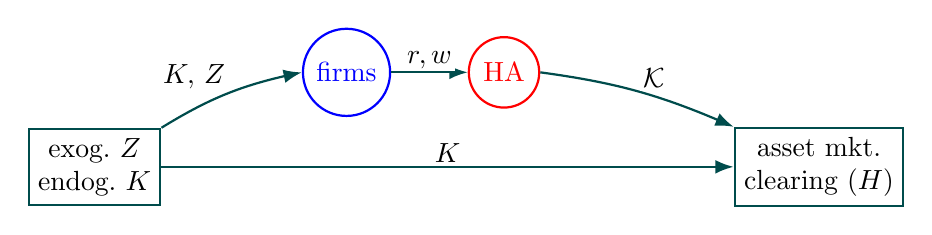
\begin{tikzpicture}[
            >=Latex,
            box/.style={draw=teal!60!black, thick, rectangle,  align=center},
            bluecirc/.style={draw=blue, thick, circle, align=center, text=blue},
            redcirc/.style={draw=red, thick, circle, align=center, text=red},
            flow/.style={->, thick, draw=teal!60!black},
            lab/.style={midway, fill=white, inner sep=1pt}
        ]

        % nodes
        \node[box] (leftbox) at (0,0) {exog.\ $Z$ \\ endog.\ $K$};
        \node[bluecirc] (firms) at (3.2,1.2) {firms};
        \node[redcirc] (ha) at (5.2,1.2) {HA};
        \node[box] (market) at (9.2,0) {asset mkt. \\ clearing $(H)$};

        % arrows
        \draw[flow] (leftbox.north east) to[bend left=10] node[lab, above left] {$K,\,Z$} (firms.west);
        \draw[flow] (firms.east) -- node[lab, above] {$r,w$} (ha.west);
        \draw[flow] (ha.east) to[bend left=8] node[lab,above right] {$\mathcal{K}$} (market.north west);
        \draw[flow] (leftbox.east) -- node[lab, above] {$K$} (market.west);

    \end{tikzpicture}
    \end{center}
    \begin{itemize}
        \item Define $\mathbf{J}^{o,i}$ to be the \alert{total derivative} of $o$ along the DAG with respect to the exogenous or endogenous variable $i$ (distinct from the block Jacobian $\mathcal{J}^{o,i}$).
        \item Here, for example, $\mathbf{J}^{r,K}$ equals $\mathcal{J}^{r,K}$, etc.: the direct effect is the only effect.
        \item Then we need the chain rule. For instance:
              \[
                  \textcolor{red}{ \mathbf{J}^{\mathcal{K},K}} = \textcolor{red}{\mathcal{J}^{\mathcal{K},r}} \textcolor{blue}{\mathbf{J}^{r,K}} + \textcolor{red}{\mathcal{J}^{\mathcal{K},w}} \textcolor{blue}{\mathbf{J}^{w,K}}
              \]
        \item Finally, we obtain $\mathbf{H}_K$ and $\mathbf{H}_Z$; then $\mathbf{G}^{K,Z} \equiv -\mathbf{H}_K^{-1}\mathbf{H}_Z$ gives the general equilibrium map from $Z$ to $K$, and all $\mathbf{G}^{o,Z}$ are determined from it.
    \end{itemize}
\end{frame}

\begin{frame}{DAG}{General case: solving with forward accumulation}
    \begin{itemize}
        \item Initialize $\mathbf{J}^{i,i}$ as the identity for all exogenous or unknown $i$.
        \item Evaluate the chain rule following a topological sort:
              \[
                  \mathbf{J}^{o,i} = \sum_{m \in I_b} \mathcal{J}^{o,m} \mathbf{J}^{m,i}
              \]
              on blocks $b$ to get $\mathbf{H}_U = \mathbf{J}^{H,U}$ and $\mathbf{H}_Z = \mathbf{J}^{H,Z}$.
        \item This is called ``forward accumulation'' in the algorithmic differentiation literature.
        \item Compute the general equilibrium mapping:
              \(
              \mathbf{G}^{U,Z} = -\mathbf{H}_U^{-1} \mathbf{H}_Z
              \)
        \item Then do forward accumulation again:
              \[
                  \mathbf{G}^{o,Z} = \sum_{m \in I_b} \mathcal{J}^{o,m} \mathbf{G}^{m,Z}
              \]
              to get general equilibrium mappings $\mathbf{G}^{o,Z}$ from shocks $dZ$ to all variables $o$ of interest.
        \item This gives impulse responses to every shock simultaneously.
    \end{itemize}
\end{frame}



\begin{frame}{Determinacy and Large-Scale Solutions in the Sequence Space}{From truncated Jacobians to quasi-Toeplitz operators}
\small
\begin{block}{Main result}
For stationary models, sequence-space Jacobians admit the decomposition
\[
J = T(j) + E
\]
where $T(j)$ is Toeplitz and $E$ is a compact correction.
\end{block}

\begin{itemize}
    \item Far from date $0$, the Jacobian is approximately translation invariant:
    \[
    J_{t,s}\approx j_{t-s}.
    \]
    \item $E$ captures \alert{missing anticipation}: shocks near $t=0$ are not fully anticipated in the past.
    \item This applies to stationary heterogeneous-agent blocks \& stable linear expectational systems.
\end{itemize}

\end{frame}

\begin{frame}{Determinacy and Large-Scale Solutions in the Sequence Space}{Large-scale solution}
\small
We need to solve $Jx = y$. Instead of directly inverting a huge truncated matrix,

\begin{block}{Preconditioned iterative solution}
Use an approximate inverse
\[
P \approx T(j^{-1})+\widetilde E
\]
as a preconditioner, and solve the truncated system iteratively (e.g. GMRES).
\end{block}

\begin{itemize}
    \item Toeplitz part is cheap to apply/store:
    \[
    T_T(j^{-1}) \quad \text{via FFT in } O(T\log T).
    \]
    \item Compact correction is compressed in low rank:
    \[
    \widetilde E\approx U_{T,r}V_{T,r}' ,\qquad r\ll T.
    \]
    \item This reduces truncation error and avoids direct $nT\times nT$ inversion.
\end{itemize}

\end{frame}

\begin{frame}{Determinacy and Large-Scale Solutions in the Sequence Space}{Takeaway \cite{auclert2025determinacy}}
\small
\begin{alertblock}{What this adds to SSJ}
The paper extends SSJ in two directions:
\begin{itemize}
    \item \alert{theory}: existence / uniqueness / determinacy;
    \item \alert{computation}: very large sequence-space systems can be solved quickly.
\end{itemize}
\end{alertblock}
\end{frame}

\begin{frame}{2nd SSJ}{From certainty equivalence to certainty correspondence}
\small

\begin{block}{Known result}
At first order, which is the usual certainty equivalence
\[
\text{perfect-foresight sequence space}
\Longleftrightarrow
\text{linear stochastic MA}(\infty),
\]
\end{block}

Compare:

\[
X_t\!\left(\{\sigma Z_s\}_{s\ge0},D_{ss}\right)
\qquad\text{and}\qquad
\widetilde X_t=\mathcal X_t(\sigma,\epsilon_t,\epsilon_{t-1},\ldots;\{Z_s\}).
\]

\begin{alertblock}{Certainty correspondence}
\[
\text{2nd-order perfect-foresight responses}
\Longleftrightarrow
\text{coefficients of a quadratic MA}(\infty)\text{ for }\widetilde X_t.
\]
So SSJ is still enough beyond certainty equivalence.
\end{alertblock}

\end{frame}

\begin{frame}{2nd SSJ}{What corresponds to what?}
\small

Expand the stochastic solution in $\sigma$:
\[
\widetilde X_t
=
X
+\sum_{j\ge0} x_j \epsilon_{t-j}
+\frac12\!\left[
\mathcal X_{\sigma\sigma}(0)\sigma^2
+
\sum_{j,k\ge0}\mathcal X_{\epsilon_{-j}\epsilon_{-k}}(0)\,
\epsilon_{t-j}\epsilon_{t-k}
\right]
+O(\sigma^3).
\]

By symmetry in $\sigma$,
\[
\mathcal X_{\sigma\epsilon_{-j}}(0)=0.
\]

\begin{block}{Interpretation}
\begin{itemize}
    \item $\{x_j\}$ are the familiar \alert{1st-order perfect-foresight IRFs}.
    \item The quadratic coefficients
    \[
    \mathcal X_{\epsilon_{-j}\epsilon_{-k}}(0)
    \]
    are identified by \alert{2nd-order perfect-foresight responses}.
\end{itemize}
\end{block}

\end{frame}

\begin{frame}{2nd SSJ}{Why does this matter?}
\small

Rewrite the quadratic MA as
\[
\widetilde X_t \simeq
X
+\sum_{j\ge0} x_j \epsilon_{t-j}
+\frac12 \mathcal X_{\sigma\sigma}(0)\sigma^2
+\frac12\sum_{j\ge0}\mathcal X_{\epsilon_{-j}\epsilon_{-j}}(0)\epsilon_{t-j}^2
+\sum_{j<k}\mathcal X_{\epsilon_{-j}\epsilon_{-k}}(0)\epsilon_{t-j}\epsilon_{t-k}.
\]

\begin{itemize}
    \item Constant term:
    \alert{Anticipated risk}.
    \item $\epsilon^2$ terms:
    \alert{Size dependence}.
    \item $\epsilon_{t-j}\epsilon_{t-k}$ terms:
    \alert{State dependence}.
\end{itemize}

\end{frame}

\begin{frame}{2nd SSJ}{Takeaway \cite{auclert2025beyond}}
\small
\begin{alertblock}{What this adds to SSJ}
The paper extends SSJ in two directions:
\begin{itemize}
    \item Extends SSJ from linear IRFs to \alert{nonlinear, state-dependent} dynamics in sequence space;
    \item A practical framework for studying risk, nonlinear propagation, and welfare in rich heterogeneous-agent models.
\end{itemize}
\end{alertblock}
\end{frame}


\begin{frame}{SSJ in Continuous Time}{What changes relative to discrete-time SSJ?}
\small

\begin{block}{Core comparison}
Discrete-time SSJ / FNA:
\[
\text{discretize first} \;\Longrightarrow\; \text{differentiate numerically}.
\]

Continuous-time SSJ:
\[
\text{differentiate in continuous time} \;\Longrightarrow\; \text{discretize later}.
\]
\end{block}

\begin{itemize}
    \item The paper keeps the \alert{same sequence-space logic} as Auclert et al.:
    household response $\rightarrow$ distribution $\rightarrow$ fake news $\rightarrow$ Jacobian.
    \item The main change is only in the \alert{first step}:
    instead of numerically perturbing a nonlinear Euler equation,
    the household response is characterized analytically in continuous time.
\end{itemize}

\end{frame}


\begin{frame}{SSJ in Continuous Time}{Takeaway \cite{bilal2025some}}
\small

\begin{itemize}
    \item \alert{Faster}: Jacobians and impulse responses are about \alert{3 times faster} to compute.
    \item \alert{Where does the gain come from?}  
    From the policy-function step only:
    linear PDEs replace nonlinear backward solves plus numerical differentiation.
    \item \alert{Why continuous time helps}: with a binding borrowing constraint,
    the first-order condition still holds with equality, so the perturbation is cleaner.
\end{itemize}

\begin{alertblock}{Broader contribution}
The paper shows that SSJ / FNA is not tied to discrete time.  
It extends sequence-space methods naturally to \alert{continuous-time HA/HANK models},
especially environments with rich heterogeneity and occasionally binding constraints.
\end{alertblock}

\end{frame}


\subsection{Application}

\begin{frame}{Applications of the extended version of SSJ}
    \begin{itemize}
        \item Fiscal and monetary policy \cite{auclert2025fiscal,auclert2024intertemporal}
        \item Het households + het firms \cite{winberry2025new}
        \item Behavioural macro \cite{angeletos2025rank,auclert2020micro}
        \item Life-cycle model \cite{bardoczy2025sequence,bardoczy2024hank}
        \item Dynamic spatial model \cite{donald2025optimal,fan2023learning}
        \item Production network \cite{schaab2023monetary}
        \item Het banks \cite{bellifemine2022hbank}
        \item Optimal policy \cite{auclert2024optimal,mckay2022optimal}
        \item Macro labor \cite{guerreiro2024workers,kekre2023unemployment}
    \end{itemize}
\end{frame}


\section{Global Solution}

\subsection{Repeated transition method}

\begin{frame}{Repeated transition method}{From local SSJ to global sequence space}
\small

\begin{block}{What is the extension?}
Standard SSJ is mainly a \alert{local} method:
\[
\text{1st-order} \;+\; \text{perfect foresight} \;+\; \text{IRFs around a reference point}.
\]

RTM extends sequence-space methods to
\[
\text{global} \;+\; \text{nonlinear} \;+\; \text{aggregate uncertainty}.
\]
\end{block}

\begin{itemize}
    \item It does \alert{not} assume perfect foresight.
    \item It does \alert{not} require a parametric law of motion for the aggregate distribution.
\end{itemize}

\end{frame}

\begin{frame}{Repeated transition method}{Why ``repeated transitions''?}
\small

To solve backward at time $t$, agents need a conditional expectation of continuation values:
\[
E_t V_{t+1}
=
\Pi_{S_t,G} V(\cdot;\Phi_{t+1},G)
+
\Pi_{S_t,B} V(\cdot;\Phi_{t+1},B).
\]

\begin{block}{RTM's trick}
If the simulated path is long enough, a similar aggregate state reappears.
Find a period
\[
\tilde t+1
=
\arg\min_{\tau}\|\Phi_{\tau}^{(n)}-\Phi_{t+1}^{(n)}\|
\]
with the \alert{counterfactual shock realization}.
Then use the realized value function at $\tilde t+1$ to fill in the missing continuation value.
\end{block}

\begin{itemize}
    \item Intuition: \alert{history repeats itself} along an ergodic equilibrium path.
    \item So expectations are built from \alert{repeated transitions}, not from an estimated law of motion.
\end{itemize}

\end{frame}

\begin{frame}{Repeated transition method}{Takeaway \cite{lee2025global}}
\small

\begin{itemize}
    \item \alert{More general than SSJ}: can study global nonlinear dynamics, not only local IRFs.
    \item \alert{Avoids law-of-motion misspecification}: no need to summarize the distribution with a guessed forecasting rule.
\end{itemize}

\begin{alertblock}{Takeaway}
RTM keeps the sequence-space perspective, but turns it into a \alert{global stochastic solution method}:
better suited for nonlinear state dependence, occasionally binding constraints, and models with non-trivial market clearing.
\end{alertblock}

\end{frame}

\subsection{DL in sequence space}

\begin{frame}{DL in sequence space}{From local SSJ to global sequence space}
\small

\begin{block}{What is the extension?}
Standard SSJ is mainly a \alert{local} method:
\[
\text{aggregate state} \xrightarrow{\text{Jacobian}} \text{local IRFs}.
\]
This paper instead builds a \alert{global approximation} to equilibrium in sequence space.
\end{block}

In place of a high-dimensional aggregate state such as $(z_t,\mu_t)$, use a truncated shock history
\[
z_t^T=(z_{t-T},z_{t-T+1},\ldots,z_t),
\]

\begin{itemize}
    \item The aggregate state is approximated by a \alert{sequence of past aggregate shocks},
    not by moments or histograms of the distribution.
\end{itemize}

\end{frame}

\begin{frame}{DL in sequence space}{How deep learning enters}
\small

Parameterize equilibrium objects---policies or prices---with a neural network:
\[
\mathcal N_\rho(X_t^{\text{seq},T}) \approx \text{equilibrium object at } t.
\]

Train the network to satisfy equilibrium conditions along simulated ergodic paths:
\[
\rho^*
=
\arg\min_\rho
\frac{1}{N}\sum_{t=1}^N
\big(\text{equilibrium residual}_t(\rho)\big)^2 .
\]

\begin{itemize}
    \item The network input is the truncated history of aggregate shocks.
    \item The training data come from simulated paths of the economy.
\end{itemize}

\begin{alertblock}{Compared with SSJ}
Instead of computing \alert{derivatives} around a reference point, the method directly learns
\alert{nonlinear equilibrium mappings} over the ergodic set.
\end{alertblock}

\end{frame}

\begin{frame}{DL in sequence space}{Takeaway \cite{azinovic2025deep}}
\small

\begin{itemize}
    \item \alert{Handles richer models globally}: large shocks, aggregate uncertainty, and nonlinearities.
    \item \alert{Scales to high-dimensional environments}: OLG, heterogeneous households \& firms,
    and life-cycle models with discrete retirement choice.
    \item \alert{Shape-preserving architectures}: predicted policies can be forced to be monotone
    (or concave), which makes EGM usable inside the algorithm.
\end{itemize}

\begin{alertblock}{Takeaway}
The paper extends sequence-space methods from \alert{fast local perturbation} to
\alert{global nonlinear equilibrium computation}, using deep learning to make long shock histories
computationally tractable.
\end{alertblock}

\end{frame}

\subsection{RL in sequence space}

\begin{frame}{RL in sequence space}{Agents learn prices \cite{yang2025structural}}
\small

The key step is to replace the high-dimensional distribution state by low-dimensional prices:
\[
p_t = P^*(g_t,z_t),
\qquad
\pi_t = \pi(s_t,z_t,p_t).
\]

\begin{itemize}
    \item Households care directly about \alert{prices}, not the full distribution.
    \item The algorithm therefore works with \alert{prices as state variables}.
    \item This sidesteps the \alert{Master equation}, where the distribution would enter the Bellman equation.
\end{itemize}

\end{frame}




\section{Reference}

\begin{frame}[allowframebreaks]{Reference}
    \nocite{*}
    \scriptsize
    \setbeamertemplate{bibliography entry title}{\space}
    \setbeamertemplate{bibliography entry location}{\space}
    \setbeamertemplate{bibliography entry note}{\space}
    \bibliographystyle{apalike}

    \bibliography{reference}
\end{frame}


\end{document}
